\setcounter{secnumdepth}{3}
\section{Moduł R\_PEAKS}
\subsection{Badania literaturowe}

Zadaniem modułu R\_PEAKS jest detekcja załamków R w elektrokardiogramie. Jest to jeden z kluczowych etapów analizy sygnału EKG. Poprawne wykrycie i oznaczenie załamków R umożliwia bowiem wykrycie pozostałych punktów charakterystycznych cyklu pracy serca. Pozwala to dalej np. na przeprowadzenie dokładnej analizy zmienności rytmu serca. Załamki R są częścią tzw. zespołu QRS, który został przedstawiony na rysunku \ref{fig:RPQRS}.
\begin{figure}[H]
\centering

\includegraphics[scale=0.7]{R_PEAKS/img/qrs_class}
\caption{Fragment sygnału EKG z zaznaczonym zespołem QRS (QRS Complex)}
\label{fig:RPQRS}
\end{figure}
Zespół QRS tworzą trzy sąsiadujące ze sobą punkty elektrokardiogramu, które składają się na wychylenie w kształcie wąskiego impulsu. Załamek Q to pierwsze ujemne wychylenie elektrokardiogramu, załamek R to pierwsze dodatnie wychylenie elektrokardiogramu, a załamek S to ostatnie ujemne wychylenie elektrokardiogramu w zespole QRS.

Zespół QRS jest odzwierciedleniem elektrycznej aktywności serca podczas skurczu komorowego. Reprezentuje on pobudzenie, czyli depolaryzację komór serca. Zespół QRS charakteryzuje się najwyższym wychyleniem i najkrótszym czasem trwania, co sprawia, że posiada on szerokie widmo częstotliwościowe. Charakterystyczny kształt tego zespołu oraz czas jego pojawiania się dostarcza najwięcej informacji diagnostycznych o bieżącym stanie serca i dlatego też jest punktem wyjściowym do klasyfikacji schematu cyklu sercowego. Służy też jako podstawa do automatycznego określania rytmu. Wykrycie zespołu QRS dostarcza podstawowych zasad i informacji dla prawie wszystkich automatycznych algorytmów analizy EKG. Czas trwania oraz wysokość zespołu QRS jest zależny od wielu czynników. Przyjmuje się jednak, że dla dorosłego i zdrowego człowieka średni czas trwania zespołu powinien wynosić od 0,06 s do 0,10 s. Wysokość sygnału zaś powinna mieścić się między 0,7 mV a 1,8 mV.

Detekcja załamków R wciąż jest przedmiotem wielu badań oraz licznych prac naukowych. Nie opracowano do tej pory metody, która gwarantowałaby stuprocentową skuteczność działania. Istnieją jednak algorytmy, które zapewniają ponad dziewięćdziesięciodziewięcio procentową skuteczność. Najpowszechniej stosowanym algorytmem jest algorytm Pan-Tompkins. Bazuje on na analizie odpowiednio przefiltrowanego oraz uśrednionego sygnału EKG. Algorytm ten łatwo adaptuje się do dynamiki sygnału. Dzięki temu jest bardzo skuteczny nawet w przypadku nieregularnej pracy serca. Ponadto metoda ta bardzo dobrze spisuje się w systemach czasu rzeczywistego. Wśród pozostałych algorytmów dużą popularnością cieszą się algorytmy oparte na przekształceniach Hilberta oraz transformacji falkowej. Przedmiotem obecnych badań są też metody, które łączyłyby te dwa algorytmy. Pozostałymi algorytmami detekcji załamków R są między innymi metody oparte na sieciach neuronowych, algorytmach genetycznych czy procesach stochastycznych.
\subsection{Koncepcja proponowanego rozwiązania}

W trakcie realizacji modułu R\_PEAKS zdecydowano się na implementację trzech algorytmów detekcji załamków R:
\begin{itemize}
\item algorytm Pan - Tompkins,
\item algorytm bazujący na przekształceniach Hilberta,
\item algorytm bazujący na transformacji falkowej.
\end{itemize}
\subsubsection{Algorytm Pan - Tompkins}

Algorytm ten można podzielić na dwa etapy. Pierwszym jest odpowiednie przygotowanie sygnału poprzez przefiltrowanie go oraz późniejsze jego uśrednienie. Drugim etapem jest znajdowanie załamków R we wcześniej przygotowanym sygnale. Na rysunku ~\ref{fig:RPPTA} przedstawiono schemat blokowy pierwszego etapu algorytmu.
\begin{figure}[H]
\centering
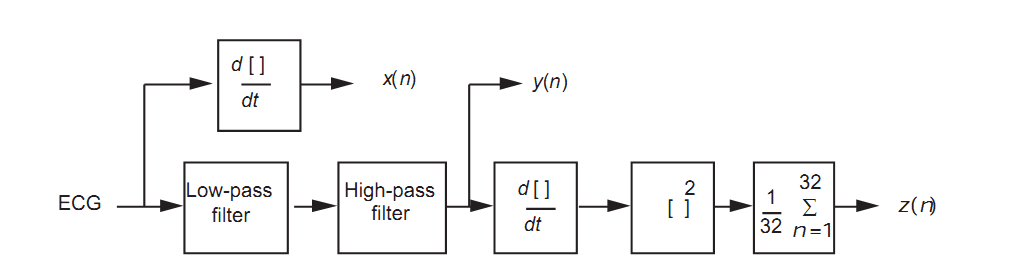
\includegraphics[scale=0.4]{R_PEAKS/img/pan_tompkins_alg}
\label{fig:RPPTA}
\caption{Kolejne etapy algorytmu Pan - Tompkins przygotowujące sygnał do detekcji załamków R}
\end{figure}
\begin{enumerate}[I.]
\item Przepuszczenie sygnału przez filtry dolno i górnoprzepustowy.
\item Różniczkowanie

Celem różniczkowania sygnału jest wytłumienie komponentów niskoczęstotliwościowych oraz wzmocnienie komponentów wysokoczęstotliwościowych charakterystycznych dla zespołów QRS. W tej fazie skorzystano z różniczkowania pięciopunktowego opisanego wzorem:
\begin{equation}
y(nT)=\frac{1}{8}[-x(nT-2T)-2x(nT-T)+2x(nT+T)+x(nT+2T)]
\end{equation}
\item Potęgowanie

Potęgowanie sygnału ma na celu jeszcze większe wzmocnienie próbek sygnału odpowiadających zespołom QRS oraz wytłumienie pozostałych próbek sygnału. Ponadto potęgowania zapewnia nieujemność sygnału.
\begin{equation}
y(nT)=[x(nT)]^2
\end{equation}
\item Całkowanie

Całkowanie sygnału w ruchomym oknie ma na celu jego wygładzenie oraz uzyskanie pojedynczej "fali" w obrębie zespołu QRS. Całkowanie sygnału wyraża się następującym wzorem:
\begin{equation}
y(nT)=\frac{1}{N}\sum\limits_{i=nT-NT}^{nT} x(i)
\end{equation}
Gdzie N to szerokość okna, którą należy odpowiednio dobrać w zależności od częstotliwości próbkowania. Należy mieć tu na uwadze fakt, że zbyt duża wielkość okna spowoduje zlanie się dwóch fal, a zbyt mała z kolei skutkować będzie utworzeniem zbyt dużej liczby fal.
\item Progowanie i detekcja załamków R

W trakcie pracy algorytmu odnajdywane są kolejne maksima lokalne, którą mogą być oznaczone jako załamek R lub jako szum. Wykorzystywane są przy tym dwa progi: THRESHOLD1 i THRESHOLD2. Są one na bieżąco aktualizowane na podstawie estymaty amplitudy załamków R (SPK) i szumu (NPK). Dodatkowo wykorzystywana jest technika searchback z parametrem RRMISSEDLIMIT, który wyznaczany jest na podstawie różnic między kolejnymi załamkami R. Poniżej przedstawiono reguły detekcji załamków R:

\begin{algorithmic}
\If {załamek R wykryto w czasie maksymalnie 200 ms od ostatniego załamka R \textbf{AND} amplituda nowego załamka jest mniejsza od poprzedniego wykrytego}
    \State odrzuć załamek
\ElsIf {nowy załamek R wykryto w czasie ponad 200 ms, a mniej niż 360 ms od ostatniego załamka \textbf{AND} nachylenie sygnału przy nowym maksimum jest przynajmniej równe połowie nachylenia dla poprzedniego maksimum}
    \State dodaj załamek
\ElsIf {wartość wykrytego maksimum jest większa niż THRESHOLD1}
	\State dodaj załamek
\ElsIf{załamek R nie został wykryty przez okres RRMISSEDLIMIT \textbf{AND} w ciągu tego czasu zostały znalezione maksima większe niż THRESHOLD2}
	\State dodaj jako załamek największe znalezione maksimum
\EndIf
\end{algorithmic}
%\begin{itemize}
%\item Jeżeli nowy załamek R wykryto w czasie maksymalnie 200 ms od ostatniego załamka R i amplituda nowego załamka jest mniejsza od poprzedniego wykrytego to ten załamek jest odrzucany.
%\item Jeżeli nowy załamek R wykryto w czasie ponad 200 ms, a mniej niż 360 ms od ostatniego załamka sprawdza się, czy maksymalne nachylenie sygnału przy nowym maksimum jest przynajmniej równe połowie nachylenia dla poprzedniego maksimum. Jeżeli nie, to przyjmuje się, że maksimum jest szumem, np. załamkiem T.
%\item Jeżeli wartość wykrytego maksimum jest większa niż THRESHOLD1, to uznaje się to maksimum za załamek R, w przeciwnym razie jest to szum.
%\item Technika searchback: Jeżeli załamek R nie został wykryty przez okres RRMISSEDLIMIT, a w ciągu tego czasu zostały znalezione maksima większe niż THRESHOLD2, to największe z nich traktowane jest jako załamek R.
%\end{itemize}
W takcie działania algorytmu konieczna jest aktualizacja progów. Są one aktualizowane na podstawie wartości parametrów SPK i NPK, których początkowe wartości są następujące:
\begin{itemize}
\item SPK = średnia z ośmiu maksimów z pierwszych ośmiu sekund badania,
\item NPK = 0.
\end{itemize}
Wartości tych parametrów są aktualizowane w następujący sposób:
\begin{algorithmic}
\If {załamek R został wykryty za pomocą porównania z THRESHOLD1}
    \State $SPK \gets 0.125 PEAK + 0.875 SPK$
\ElsIf {załamek R został wykryty za pomocą porównania z THRESHOLD2}
	\State $SPK \gets 0.250 PEAK + 0.750 SPK$
\Else 
	\State $NPK \gets 0.125 PEAK + 0.875 NPK$
\EndIf
\end{algorithmic}
%\begin{itemize}
%\item jeżeli załamek R został wykryty za pomocą porównania z THRESHOLD1 
%\newline
%SPK = 0.125 PEAK + 0.875 SPK,
%\item jeżeli załamek R został wykryty za pomocą porównania z THRESHOLD2 
%\newline
%SPK = 0.250 PEAK + 0.750 SPK,
%\item jeżeli został wykryty szum
%\newline
%NPK = 0.125 PEAK + 0.875 NPK
%\end{itemize}
Progi natomiast są aktualizowane w następujący sposób:
\newline
THRESHOLD1 = NPK+ 0.25 (SPK-NPK)
\newline
THRESHOLD2 = 0.5 THRESHOLD1

Interwały pomiędzy kolejnymi załamkami R obliczane są jako różnica wystąpienia ich czasów. Jeżeli interwał jest większy niż 0.92 RRAVERAGE2 i mniejszy niż 1.12 RRAVERAGE2, bufor interwałów jest aktualizowany o ostatnią wartość interwału i obliczana jest nowa wartość RRAVERAGE2. Wartość RRMISSEDLIMIT używana w technice searchback jest równa 1.66 RRAVERAGE2 i stanowi czas, w którym poszukiwane są zaginione maksima.
\end{enumerate}
\subsubsection{Algorytm bazujący na przekształceniach Hilberta}
Przekształcenie Hilberta to przekształcenie liniowe. Funkcji x(t) przypisywana jest funkcja xh(t) postaci:
\begin{equation}
x_H = \mathcal{H}\{x(t)\}=\frac{1}{\pi}\int_{-\infty}^\infty \frac{x(\lambda)d\lambda}{t-\lambda}
\end{equation}
W powyższym wzorze występuje dość trudna do wyliczenia niewłaściwa całka Riemanna. W takiej sytuacji należy skorzystać z transformaty Fouriera. Wzór na przekształcenie Hilberta przyjmuje wtedy postać:
\begin{equation}
x_H(t)=Im \{ \mathcal{F}^{-1} \{ \mathcal{F} \{ x(t) \}(\omega)\cdot (-j)sgn(\omega)\}  \}
\end{equation}
W pierwszym etapie algorytmu dokonujemy transformacji Hilberta całego sygnału EKG. Następnie na podstawie sygnałów x(t) oraz xh(t) wyznacza się tzw. obwiednię sygnału postaci:
\begin{equation}
\mathcal{B}(t)=\sqrt{x(t)^2+x_H(t)^2}
\end{equation}
Po wyznaczeniu obwiedni sygnału należy przystąpić do etapu progowania.

\begin{enumerate}[I.]
\item Wyznaczenie początkowej wartości progu

Pierwsza wartość progu powinna być nieco mniejsza niż maksymalna wartość sygnału B(t). Najczęściej spotykana wartość progu to ok. 0,9 wartości maksymalnej sygnału B(t).
\item Wyznaczenie wartości o jaką należy zmniejszać próg w kolejnych iteracjach

Jeżeli za M1 przyjęto maksymalną wartość sygnału B(t), a za M2 wartość minimalną tego sygnału to wartość o jaką należy zmniejszać próg w każdej iteracji wyraża się następującym wzorem:
\begin{equation}
fi=0,01\cdot M1 \cdot x \cdot mantysa(M1-M2)
\end{equation}
\item Wyznaczenie załamków

W tym kroku należy wyliczyć ile próbek sygnału B(t) jest większych od obecnego progu. Jeżeli liczba próbek powyżej progu jest większa od ilości próbek w poprzedniej iteracji to należy zmniejszyć próg o wartość fi i ponownie policzyć próbki powyżej progu. Jeżeli ilość próbek powyżej progu się nie zmieniła to należy przerwać etap progowania.

Ostatnim etapem jest detekcja załamków R. Wyznaczone w etapie progowania próbki powyżej progu będą występować w grupach. W każdej z tych grup znajdować się będzie próbka o największej amplitudzie, która będzie szukanym załamkiem R.
\end{enumerate}
\subsubsection{Algorytm bazujący na transformacji falkowej}

Falki (z ang. wavelet) – rodziny funkcji zbioru liczb rzeczywistych w zbiór liczb rzeczywistych, z których każda jest wyprowadzona z funkcji-matki (z tzw. funkcji macierzystej) za pomocą przesunięcia i skalowania:
\begin{equation}
\psi_{j,k}(t)=\psi(2^j +k)
\end{equation}
gdzie: j,k – liczby całkowite, $\psi$ – funkcja - matka, $\psi_{j,k}$ – falka o skali j i przesunięciu k (zwana też funkcją falkową). Funkcje te dążą do zera lub po prostu wynoszą zero dla argumentów dążących do nieskończoności. Ponadto funkcje te mają energię skupioną w jednym miejscu tzn.
\begin{equation}
\int\limits_{-\infty}^{\infty} \psi(t)dt=0
\end{equation}
Transformacja falkowa dla sygnałów ciągłych jest przekształceniem całkowym:
\begin{equation}
\tilde{s}_{\Psi}=\frac{1}{\sqrt{a}}\int\limits_{-\infty}^{\infty}s(t)\Psi(\frac{t-b}{a})dt
\end{equation}
gdzie:
\begin{itemize}
\item a - parametr skali
\item b - parametr przesunięcia
\item s(t) - sygnał badany zależny od czasu t
\item $\Psi$ - funkcja falkowa
\item $\tilde{s} _\Psi$ - współczynnik falkowy zależny od parametrów a i b
\item $\Psi(\frac{t-b}{a})$ - jądro przekształcenia
\end{itemize}
Zastosowanie transformacji falkowej pozwala rozłożyć sygnał na kilka subpasm (rysunek \ref{fig:RPWS}). Następnie dobiera się odpowiednie subpasma i rekonstruuje sygnał. Tak uzyskany sygnał poddaje się takiej samej procedurze progowania i detekcji załamków R jak w przypadku wcześniej opisywanego algorytmu wykorzystującego przekształcenia Hilberta.
\begin{figure}[H]
\centering
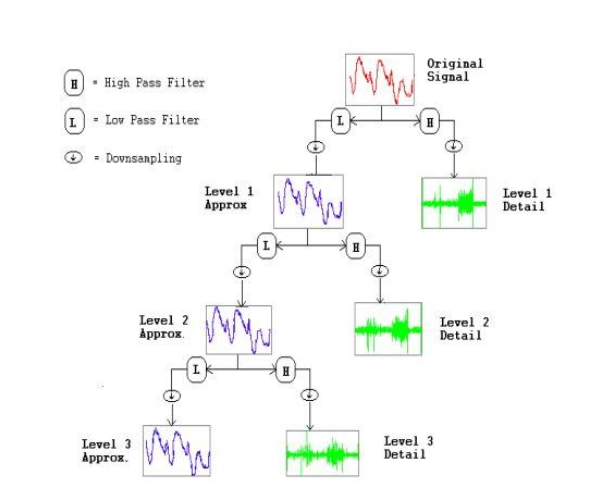
\includegraphics[scale=0.6]{R_PEAKS/img/wavelet_schema}
\caption{Dekompozycja sygnału na subpasma za pomocą transformacji falkowej}
\label{fig:RPWS}
\end{figure}

Działanie algorytmu można przedstawić w następujących krokach:
\begin{enumerate}[I.]
\item Dwukrotna dekompozycja oryginalnego sygnału z wykorzystaniem transformacji falkowej.
\item Wyszukanie próbki o największej wartości w zdekomponowanym sygnale.
\item Znalezienie wszystkich próbek o wartości nie mniejszej niż 30\% wartości próbki znalezionej w poprzednim kroku.
\item Filtracja próbek, które zostały wykryte w poprzednim kroku w celu odrzucenia tych, które należą do tego samego załamka R.
\item Znalezienie indeksów wyszukanych próbek w sygnale po transformacji i przemnożenie ich razy 4 w celu znalezienia w przybliżeniu indeksów próbek w sygnale oryginalnym, które zostały sklasyfikowane jako załamki R.
\item Wyszukanie faktycznego indeksu próbki w oryginalnym sygnale poprzez przeszukanie odpowiedniego przedziału oryginalnego sygnału wokół próbki o indeksie znalezionym w poprzednim kroku.
\end{enumerate}
\subsection{Rezultaty i wnioski}
Zaimplementowane metody w większości przypadków działają dobrze i poprawnie wykrywają załamki R. Ewentualny błąd wynosi co najwyżej kilka próbek. W przypadku sygnałów dosyć zniekształconych zdarzają się sytuacje, że zostały wykryte nadmiarowe załamki R, bądź niektóre z nich nie zostały w ogóle wykryte.

Należy jednak nadmienić, iż metody detekcji załamków R, Pan - Tompkins oraz bazująca na transformacie Hilberta, które zostały zaimplementowane w roku poprzednim przez kolegów Pawła Kasperczyka i Kamila Pękalę działają poprawnie. Z tego powodu zostały również wykorzystane w tegorocznym projekcie. Zostały wprowadzone jednak drobne modyfikacje związane z dopasowaniem tych metod pod API tegorocznego projektu, jak również pewne modyfikacje w sposobie zwracania rezultatów obliczeń funkcji składowych klasy reprezentującej moduł oraz pewne zmiany kosmetyczne związane z formatowaniem kodu. Konsekwencją wynikającą z wykorzystania zaimplementowanych już metod jest to, że są pewne różnice pomiędzy proponowanym w wcześniej rozwiązaniem a rozwiązaniem zastosowanym w programie.

W zaimplementowanej metodzie bazującej na transformacji Hilberta został zastosowany podział sygnału na przedziały. Transformacja dokonywana jest zatem na fragmencie sygnału, po czym otrzymane rezultaty sklejane są w całość. Zgodnie z informacjami zawartymi w raporcie z zeszłorocznego projektu, daje to lepsze rezultaty, niż obliczenia dokonywane na całym sygnale bez podziału na przedziały. Kolejną różnicą jest to, że nie jest obliczany pierwiastek kwadratowy, który występuje we wzorze na obwiednią sygnału. Upraszcza to obliczenia. Podyktowane jest to faktem, iż liczba rzeczywista o większej wartości ma również większy pierwiastek kwadratowy. Również sama metoda detekcji załamków R jest nieco inna niż proponowana w jednym z wcześniejszych rozdziałów. Dokonywana ona jest na podstawie przeglądu fragmentu tablicy \textit{diff} zawierającej posortowane malejąco elementy, które są większe niż $\frac{1}{21}$ maksymalnej wartości z tej. Elementy te są wkładem transformaty Hilberta w obwiednię sygnału, obliczone na podstawie wspomnianego wyżej, uproszczonego wzoru niezawierającego pierwiastka kwadratowego. Próbka sygnału wejściowego, która odpowiada aktualnie przeglądanemu elementowi tablicy, jest odpowiednio daleko od poprzednio zakwalifikowanych jako załamek R próbek, jest również traktowana jako szukany załamek. W przeciwnym przypadku jest odrzucana. Minimalna odległość między załamkami jest oszacowana na podstawie założenia, iż maksymalna częstotliwość pracy serca wynosi 220 uderzeń na minutę. Wyznaczona odległość pomnożona jest jeszcze przez współczynnik wynoszący 0,8. Szerokość fragmentu sygnału poddawanego transformacji Hilberta przyjęta została jako 200 sekund.

Bardzo ważnym elementem detekcji załamków R jest uzyskanie do analizy dobrze przefiltrowanego sygnału, pozbawionego dużych zakłóceń i szumów. Podczas testów poprawności działania modułu został przeprowadzony eksperyment polegający na detekcji załamków R w sygnale nie poddanym filtracji. Metoda Pan - Tompkins mimo wszystko dała w miarę dobre rezultaty, natomiast metoda bazująca na transformacji Hilberta kompletnie nie poradziła sobie z wykryciem pików. Prawdopodobnie główną przyczyną tego faktu jest obecność prostej i odwrotnej transformaty Fouriera w zaimplementowanej metodzie. Metoda oparta na transformacji falkowej, w zaimplementowanym w module algorytmie, wyszukuje załamki, których wartość przekracza pewien ustalony próg wyznaczony w oparciu o próbkę o największej wartości. Z tego powodu obecność zakłóceń o zbyt dużej wartości może powodować zakwalifikowanie tych zakłóceń jako nadmiarowe załamki.

Z racji, iż stosowane algorytmy przeważnie wykrywają trochę mniejszą liczbę załamków niż wynosi ona w rzeczywistości, ciężko było dokonać analizy różnic pomiędzy wynikami zwróconym przez algorytm a wynikami referencyjnymi w sposób automatyczny, przy wykorzystaniu programu. Dla wybranych sygnałów EKG zostały narysowane wykresy z naniesionymi, referencyjnymi i wyznaczonymi przez algorytmy, załamkami R. Sygnał oryginalny był filtrowany przy pomocy filtru Butterwortha. Nie zostały przeprowadzone testy dla innych metod filtracji w oparciu o założenie, że każda z tych metod daje poprawne rezultaty i wyniki detekcji załamków R powinny być podobne dla każdej z metod filtrowania sygnału.
\subsubsection{Sygnał 105}
\begin{figure}[H]
\centering
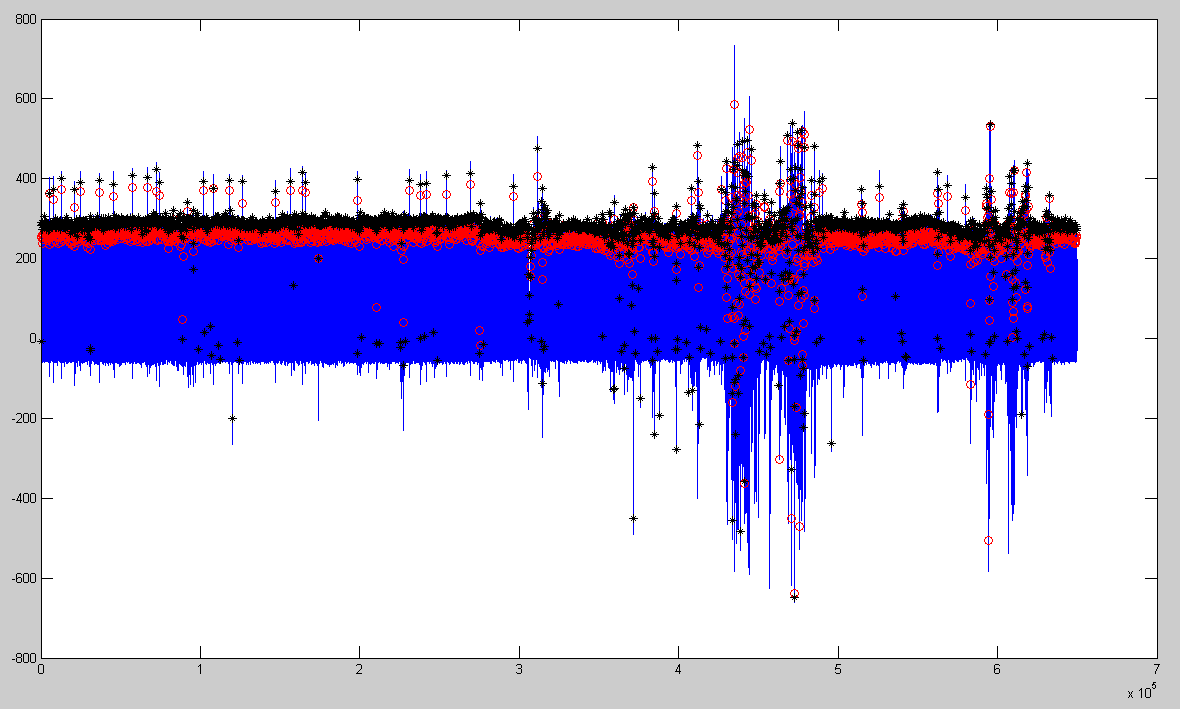
\includegraphics[scale=0.4]{R_PEAKS/img/105_hilbert_calosc}
\caption{Sygnał nr 105 z naniesionymi pikami R - Hilbert}
\label{fig:105HC}
\end{figure}
Piki referencyjne zostały oznaczone czarnymi gwiazdkami, natomiast wyznaczone przy pomocy moduły załamki R czerwonymi kółkami. Również takie same oznaczenia są przyjęte na kolejnych wykresach. Można zauważyć, że generalnie piki zostały wyznaczone całkiem dobrze, różnice są rzędu kilku próbek, co będzie widoczne lepiej na następnych wykresach. Można zauważyć, że jest parę niewykrytych w ogóle załamków.

\begin{figure}[H]
\centering
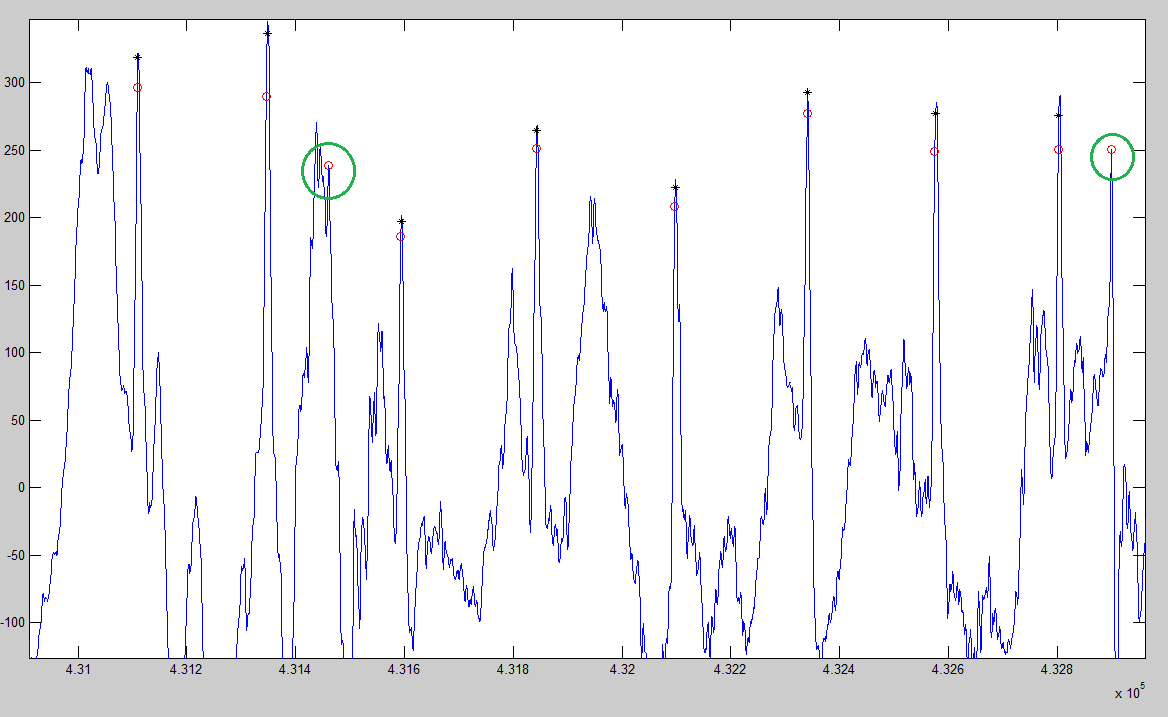
\includegraphics[scale=0.4]{R_PEAKS/img/105_hilbert_nadmiar}
\caption{Nadmiarowe załamki R - Hilbert}
\label{fig:105HN}
\end{figure}
Na powyższym wykresie widać, że mimo dosyć nieregularnego kształtu sygnału załamki zostały wykryte dosyć poprawnie. Na zielono również zaznaczono piki, które nie są zawarte w pliku z referencyjnymi załamkami.
\subsection{Literatura}